\section{ผลงานที่เกี่ยวข้อง}

\subsection{ผลงานจริงที่เกิดจากการทดลองใช้ HAPS}

จากงานนำเสนอ \cite{spacecompass}
กล่าวถึงความร่วมมือของบริษัท Airbus, NTT, DOCOMO,JSAT ในการส่งเสริมงานวิจัยและการพาณิชย์ในธุรกิจ Space RAN(Radio Access Network)
โดยเริ่มต้นจากการติดตั้งระบบ HAPS ในเครื่องบิน ชื่อว่า Zephyr ของบริษัท Airbus บินในชั้นบรรยากาศสตราโตสเฟียร์(Stratospher) 
และเริ่มการทดลองจริงโดยส่งคลื่นวิทยุไปสถานีเครือข่ายภาคพื้นดินโดยความถี่
UHF - 2GHz, 450MHz เพื่อวัดความสามารถในการกระจายสัญญาณ การทดลองนี้ใช้ระยะเวลา 18 วัน 
จึงสรุปผลการทดลองได้ว่าที่สัญญาณความถี่ 450MHz นั้นมีระยะการเชื่อมต่อสูงสุดอยู่ที่ 140 กม. \ref{fig:02-zephyr-testing}

\begin{figure}[h]
\centering
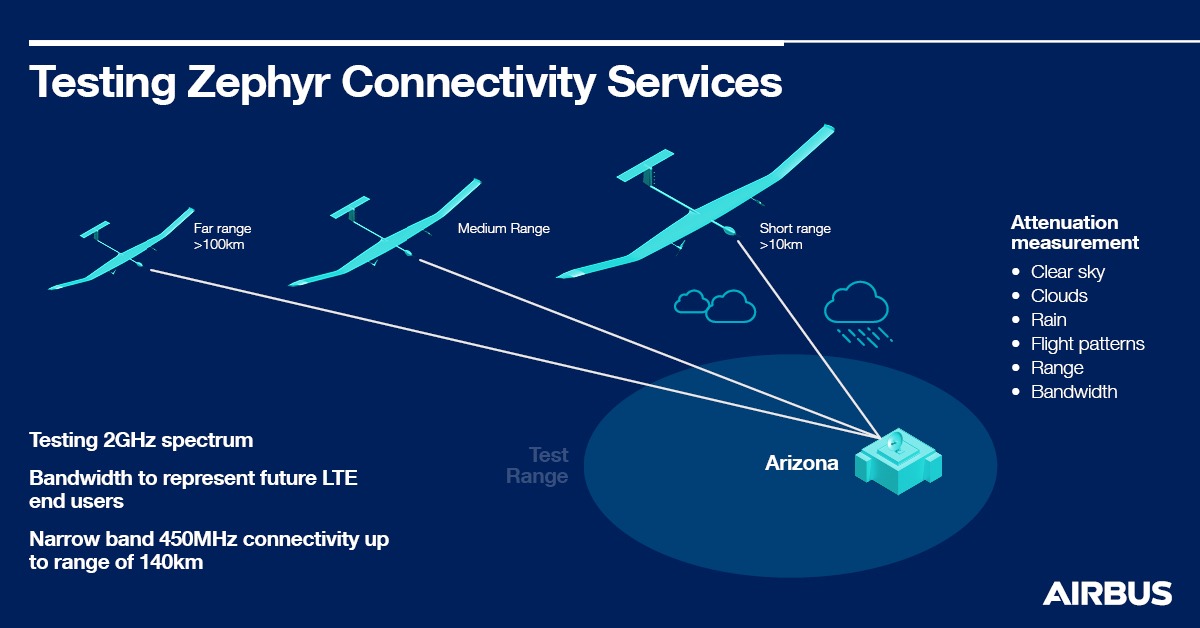
\includegraphics[width=0.5\textwidth]{02_zephys-testing.jpeg}
\caption[Testing Zephyr]{Testing Testing Zephyr Connectivity Services} \label{fig:02-zephyr-testing}
\end{figure}

จากงานวิจัย \cite[Towers]{High Altitude Platform Systems: Towers in the Skies}
นำเสนอถึงความหลากหลายของ HAPS ที่ปรับเปลี่ยนได้ตามความต้องการในด้านพื้นที่ที่สัญญาณครอบคลุม ด้วยเทคโนโลยีเสาอากาศแบบใหม่ช่วยให้กำหนดทิศทางไปยังพื้นที่เป้าหมายที่ต้องการ กลายเป็นเครือข่าย
ประเภทหนึ่งชื่อว่า Fixed wireless access (FWA) เป็นเครือข่ายสัญญาณไร้สายประเภทหนึ่งที่ให้บริการอินเทอร์เน็ตความเร็วสูงแก่ประชาชนภาคครัวเรือน ในทางทฤษฎีแล้ว
FWA ผ่าน HAPS สามารถปลดล็อคขีดจำกัดการถ่ายโอนข้อมูลสูงสุด(Capacity)และความล่าช้า(Latency)ที่ต่ำกว่าเครือข่ายจากดาวเทียม
ทำให้อาจเป็นอีกหนึ่งทางเลือกนอกจากเครือข่ายสัญญาณแบบไฟเบอร์(Fibre-based) \ref{fig:02-wireless-vs-satellite}

\begin{figure}[h]
\centering
\includegraphics[width=0.5\textwidth]{02_wireless-vs-satellite-Internet.jpg}
\caption[wireless vs satellite]{Fixed wireless Internet compare with Satellite Internet} \label{fig:02-wireless-vs-satellite}
\end{figure}

\subsection{การประยุกต์ใช้ ICM}

จากงานวิจัยของ \cite{liu2021interference}
นำเสนอถึงวิธีการแทรกคลื่นสัญญาณ(Interference Coordination Method - ICM) เข้าไประหว่างคลื่นสัญญาณของ HAPS กับ สถานีเครือข่ายภาคพื้นดิน โดยมีเงื่อนไขต่อไปนี้
\begin{itemize}
    \item คำนึงถึงการกระจายปริมาณรับส่งข้อมูลเป็นหลัก 
    \item ประสิทธิภาพที่ได้โดยเทียบจากปริมาณพลังงาน,ทรัพยากรที่เสียไปและปริมาณข้อมูลที่เคลื่อนที่ผ่านเครือข่าย ณ เวลาที่กำหนด (Traffic Load)
\end{itemize}
